\section{Device Features}
In the following section the features of the DualSense controller will be explained.

\subsection{Overview}
\begin{itemize}
	\item \textbf{Connectivity} The DualSense controller can be used via a USB C cable or Bluetooth.
	\item \textbf{Integrated battery} Featuring an integrated battery, the DualSense controller is best used via Bluetooth. The controller can be charged via USB C.
\end{itemize}

\begin{figure}[H]
    \centering
    \subfloat[\centering Front View]{{\includegraphics[width=5cm]{frontView} }}
    \qquad
    \subfloat[\centering Rear View]{{\includegraphics[width=5cm]{rearView} }}
    \caption{The DualSense controller}
\end{figure}

The DualSense controller conatins the following features:
\begin{itemize}
	\item Two XY-Axis analog sticks with integrated push button.
	\item Two adaptive triggers (are able to provide resistance feedback).
	\item Two shoulder buttons.
	\item Directional-pad with the ability to press up to two neighboring buttons simultaneously.
	\item Four circular face buttons (Square, Cross, Circle and Triangle).
	\item Dual-touch touchpad with integrated push button, surrounded by an RGB-LED lightbar and a five LED player indicator on the bottom.
	\item Menu, share, PlayStation and microphone mute button.
	\item 6-Axis IMU (gyroscope and  accelerometer).
	\item Left and right rumble motors (Hard and Soft respectively). Can alternatively used as haptic feedback (not supported).
	\item Integrated speaker and microphone (both not supported).
	\item Stereo audio jack (not supported).	
\end{itemize}

\subsection{Feature List}

\paragraph{Analog sticks}
Each analog stick has two axes with 8-Bit precision. The analog sticks will return to their centered position if released. Output values are mapped to the range $-128$ to $127$ where $0$ indicates the stick is centered. The minimum values are located on the left/bottom of the respective X/Y-Axis and maximum values at the right/top. For best results the analog values should incorporate a dead zone as analog sticks are notorious for not resetting exactly to $R_{xy}(0; 0)$. Same goes for the extreme values witch will also be off and not be exactly $T_{xy}(0; 127)$, $L_{xy}(-128; 0)$, etc..
\begin{figure}[H]
    \centering
    \subfloat{{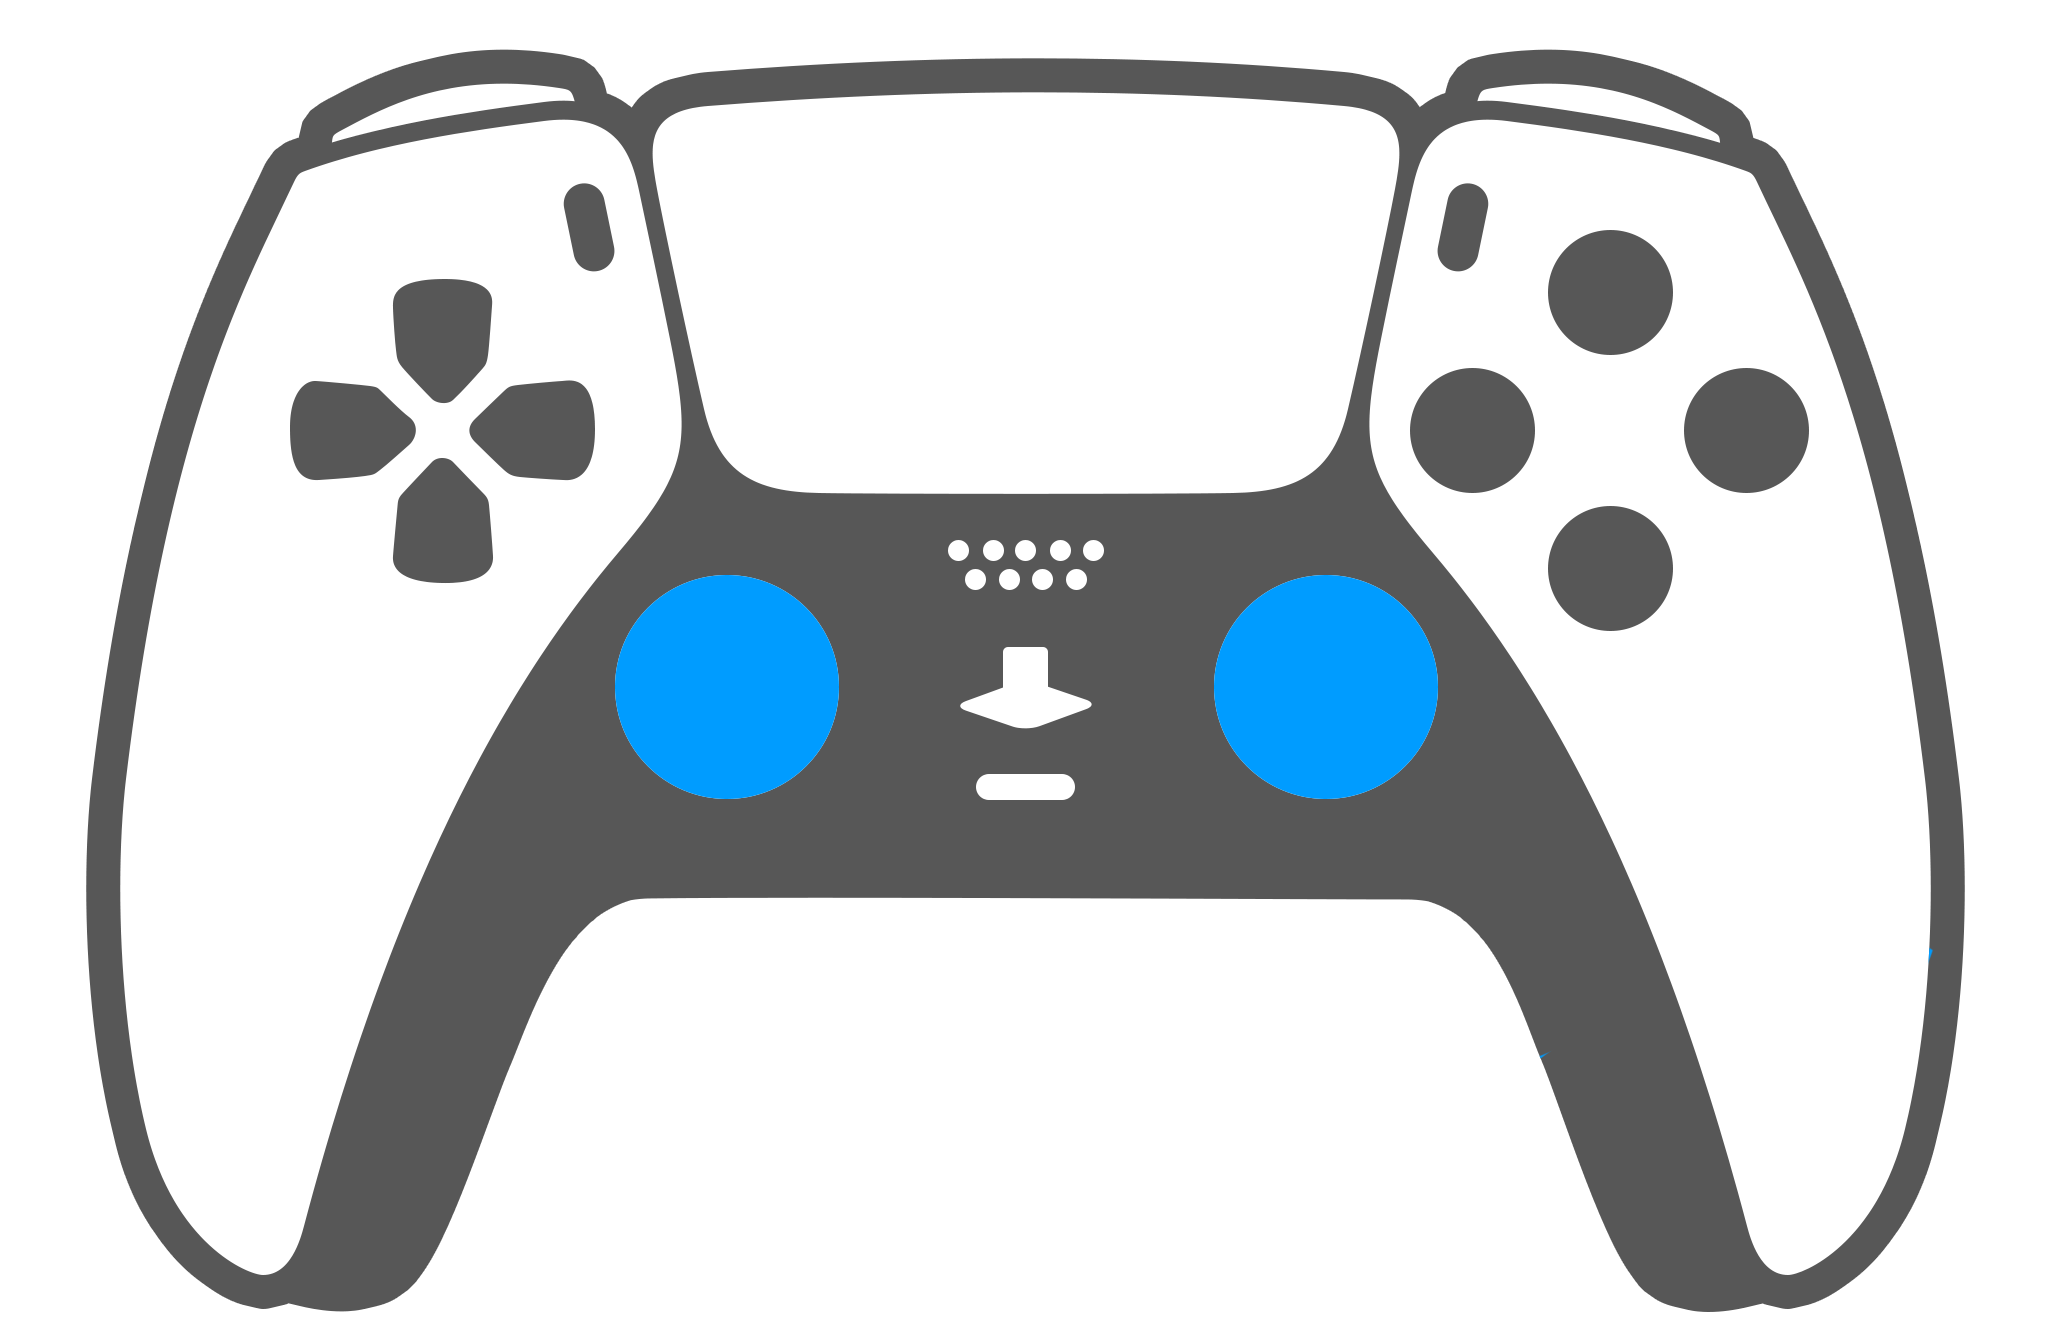
\includegraphics[width=8cm]{frontView_sticks} }}
    \caption{Analog sticks}
\end{figure}

\paragraph{Adaptive trigger}
The DualSense controller features two 8-Bit analog triggers. It is possible to read each trigger's value as an 8-Bit continuous value (0-255) or alternatively as a binary button input. Aside of the normal trigger operation, the adaptive triggers can be configured to simulate various force feedback effects, e.g. to simulate a gun trigger.
\begin{figure}[H]
    \centering
    \subfloat{{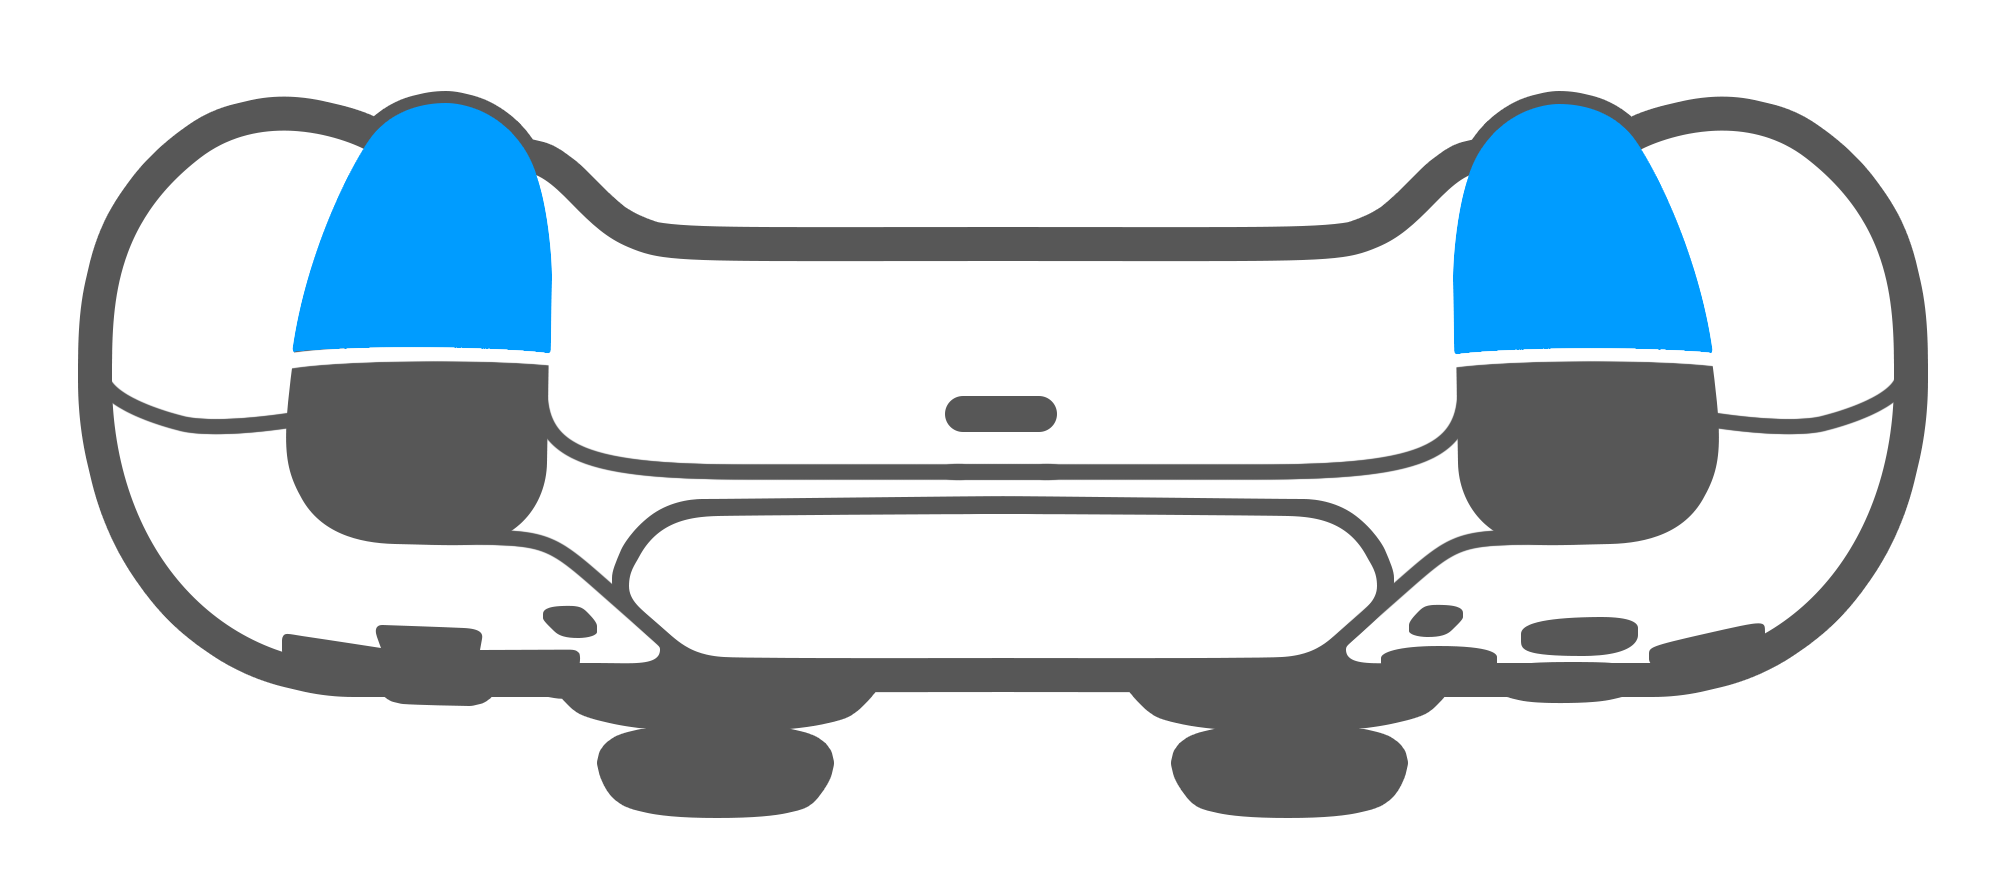
\includegraphics[width=8cm]{rearView_trigger} }}
    \caption{Adaptive triggers}
\end{figure}

\paragraph{Bumpers}
The two L/R Bumpers located above the adaptive triggers can be read as binary button inputs.
\begin{figure}[H]
    \centering
    \subfloat{{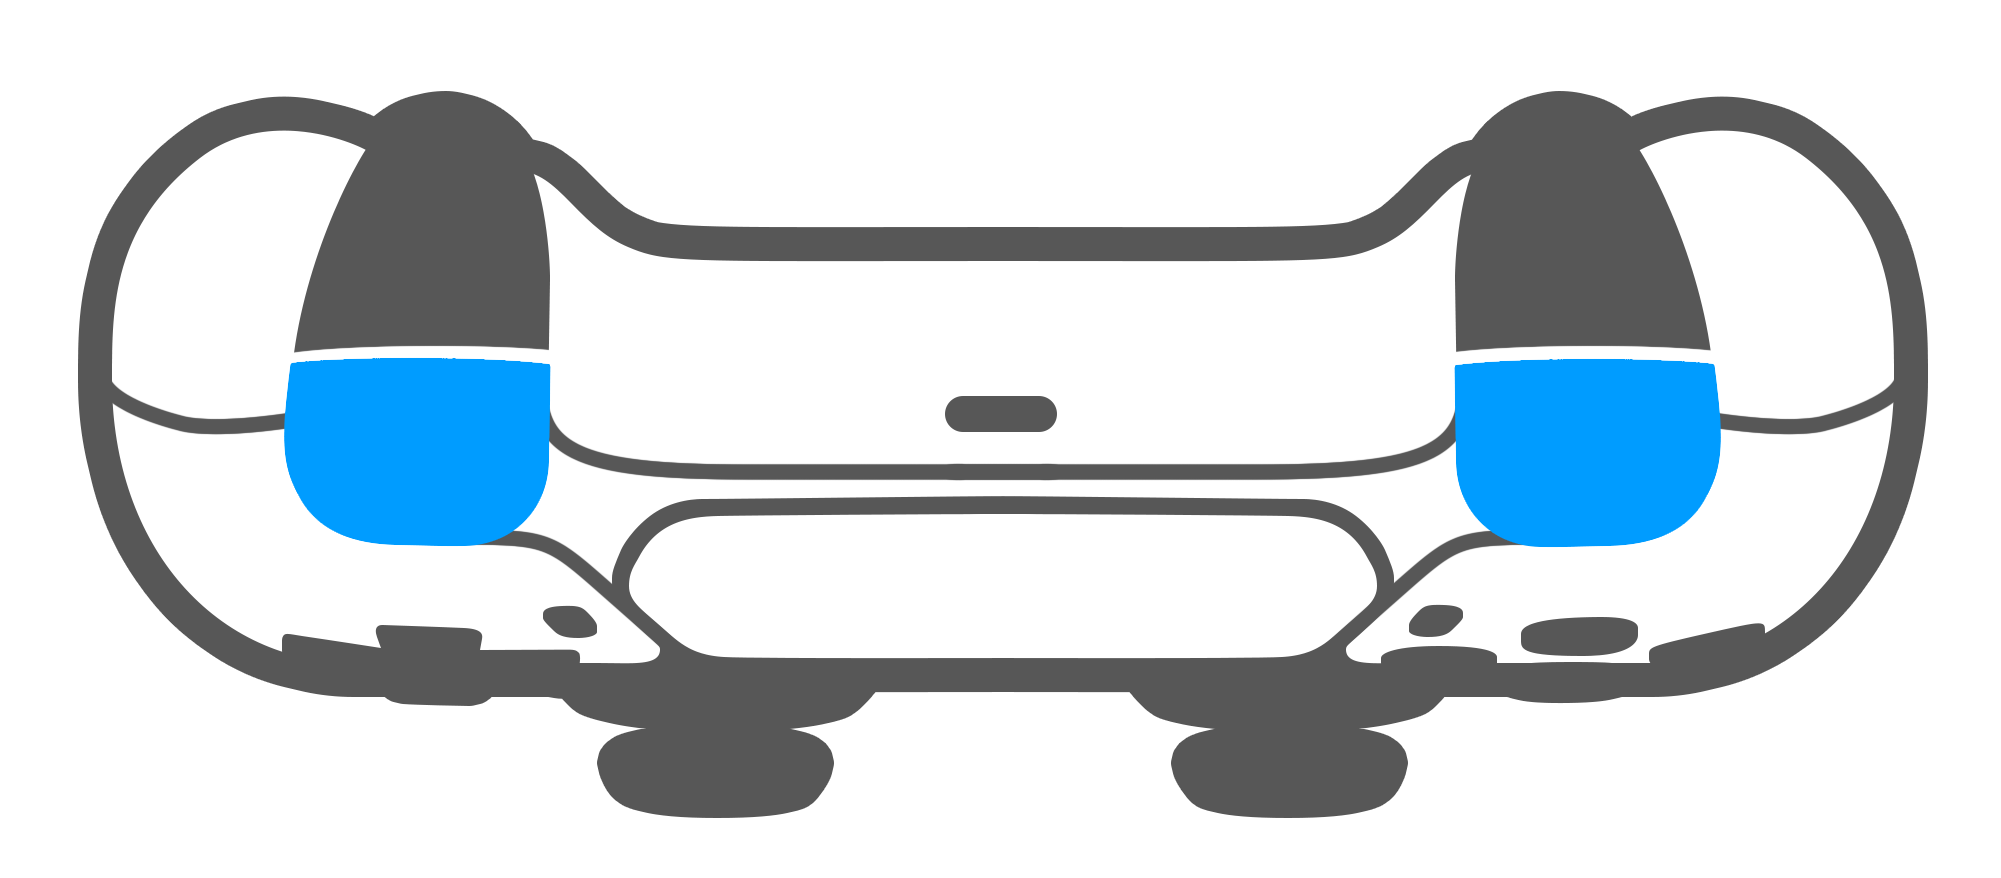
\includegraphics[width=8cm]{rearView_bumpers} }}
    \caption{L/R Bumpers}
\end{figure}

\paragraph{DPAD and PS Buttons}
The DualSense controller face features a four-directional DPAD and the well known PlayStation buttons: Square, Cross, Circle and Triangle. The DPAD is capable of registering two simultaneously pressed buttons, however the two buttons must be neighbors. The PS-Buttons are registered as four individual binary values and can all be pressed simultaneously.
\begin{figure}[H]
    \centering
    \subfloat{{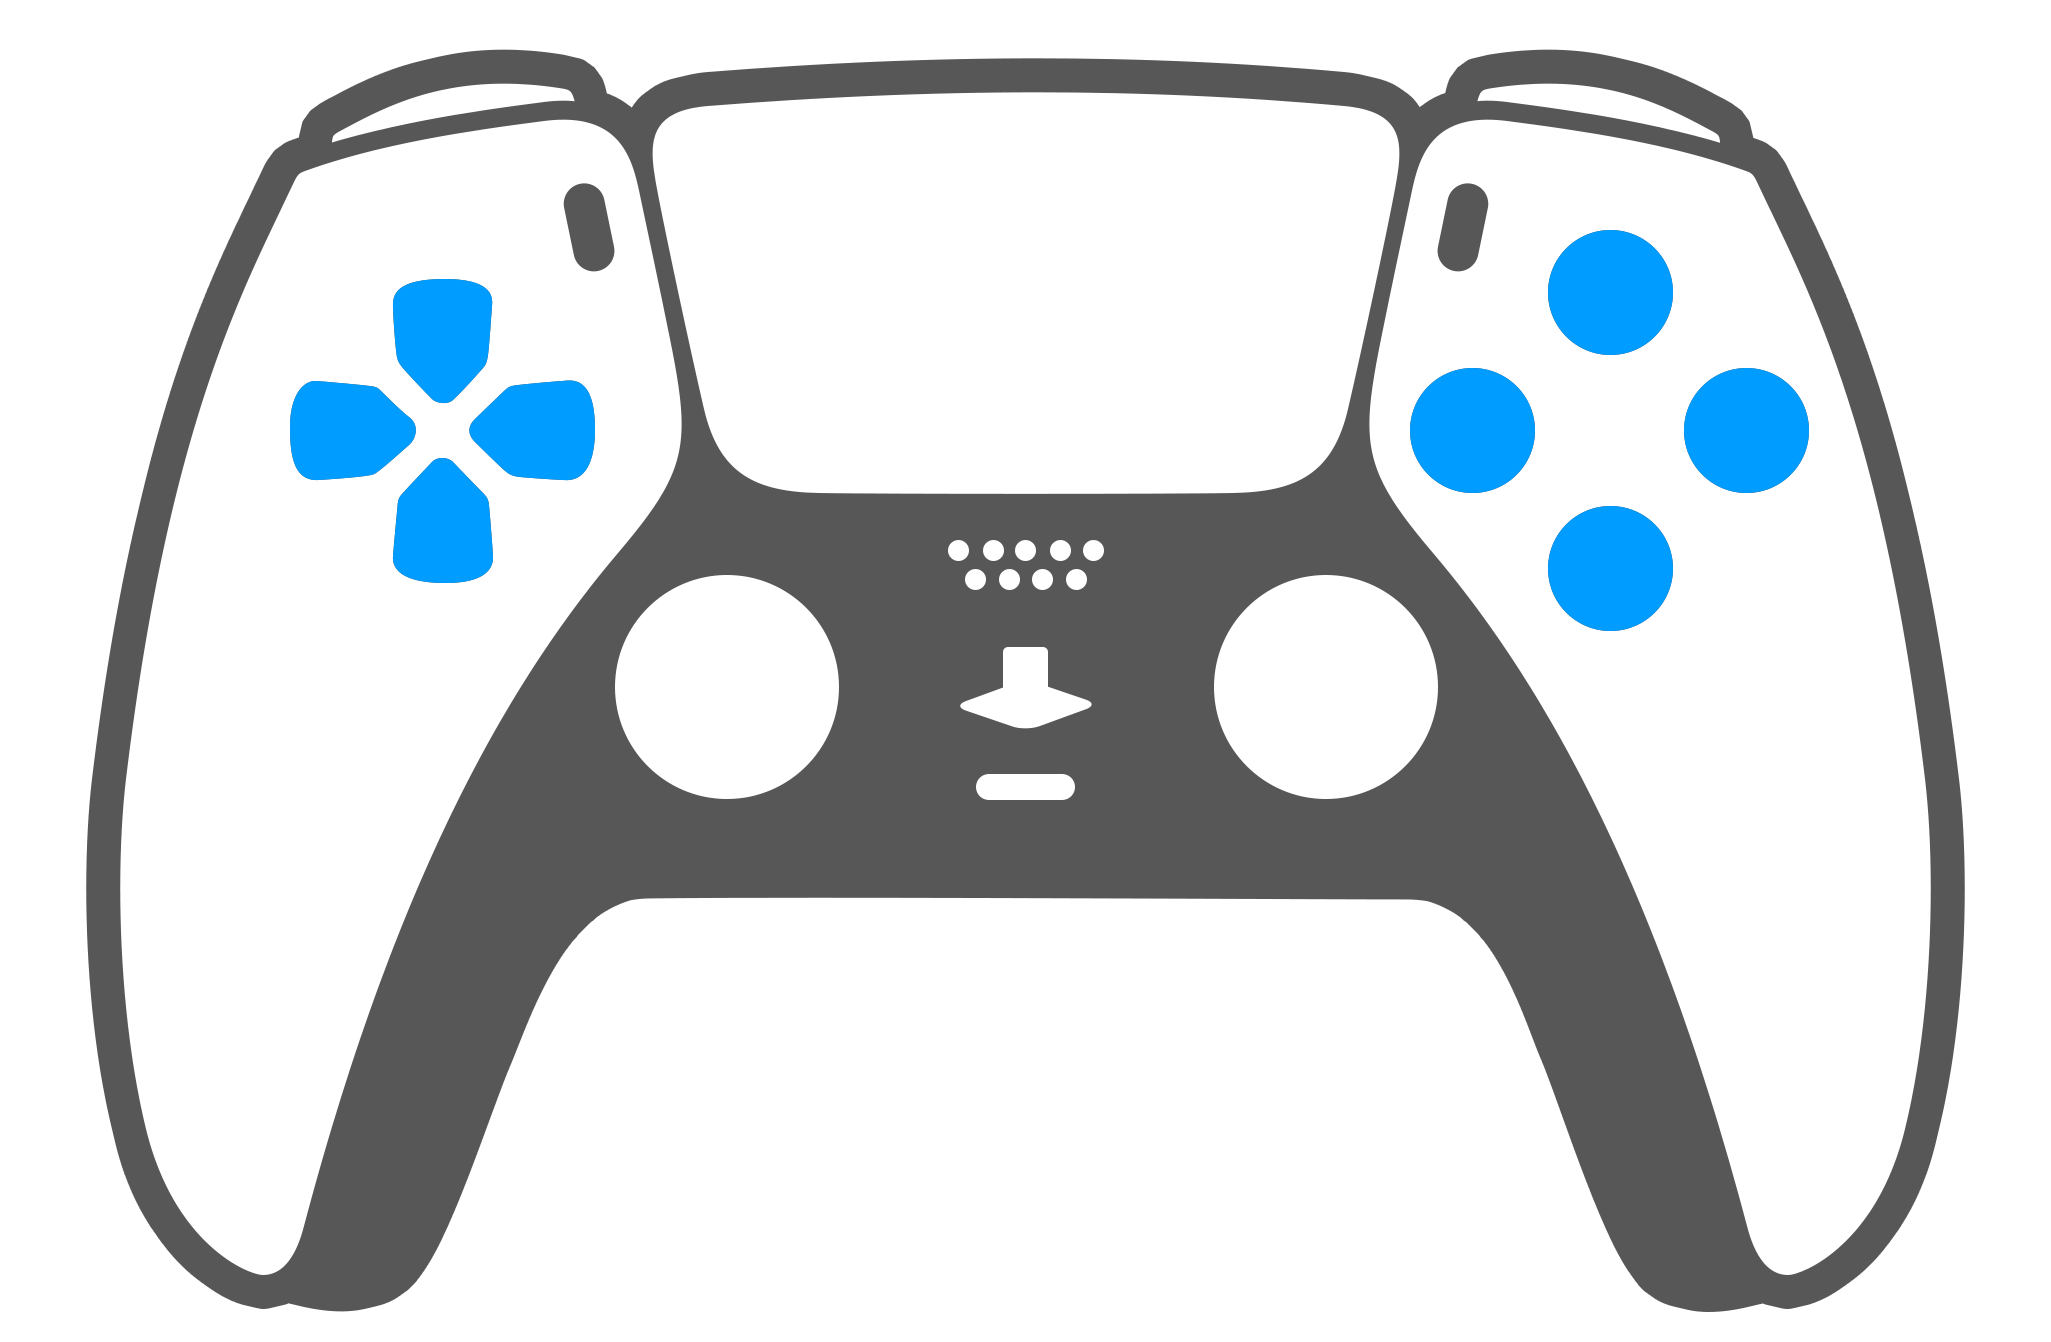
\includegraphics[width=8cm]{frontView_mainbtn} }}
    \caption{DPAD and PS-Buttons}
\end{figure}

\paragraph{Other Buttons}
The DualSense controller feature several more buttons. Thees are:
\begin{itemize}
	\item \textbf{Menu button} Often used to open the in-game menu.
	\item \textbf{Share button} Often used to open the in-game photo mode.
	\item \textbf{PlayStation button} Can be used to open a in-game overlay (also used to shutdown the device in Bluetooth mode if long-pressed).
	\item \textbf{Mic button} Should be used to mute the microphone.
\end{itemize}
All the listed buttons are readable as individual binary values.
\begin{figure}[H]
    \centering
    \subfloat{{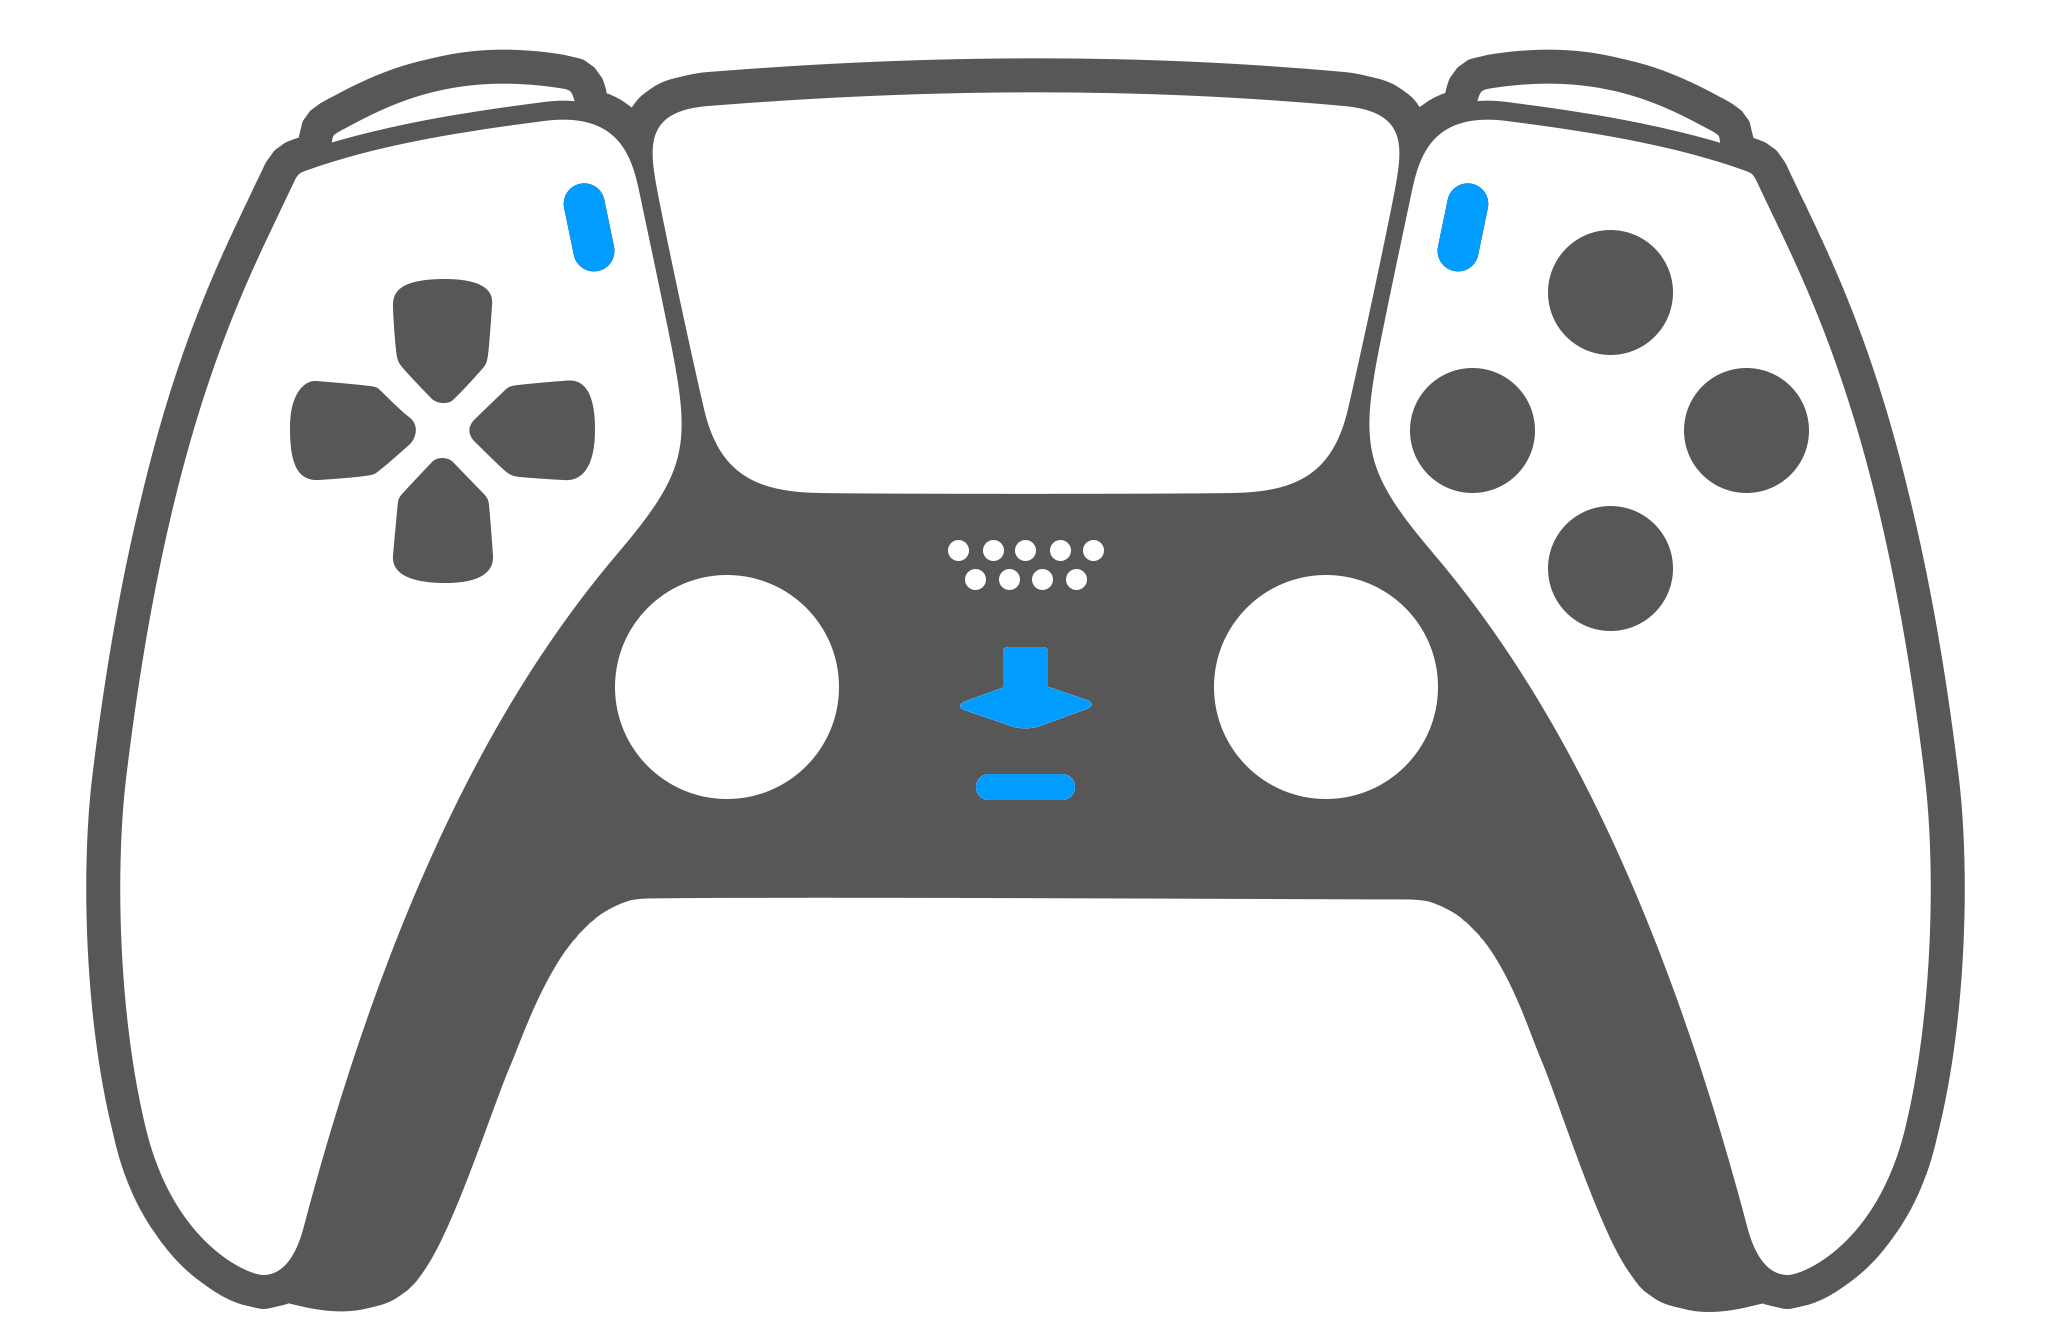
\includegraphics[width=8cm]{frontView_other} }}
    \caption{Left to right, top to bottom: Share, Menu, PlayStation and Mic Button}
\end{figure}

\paragraph{Touch Pad}
The touch-pad and the surrounding lightbar have featuring several functions:
\begin{itemize}
	\item \textbf{Dual finger touch} The touch-pad itself is able to track two fingers simultaneously as well as know how many times it has been touched (*loops after 127 touches).
	\item \textbf{Integrated push button} The touch-pad includes a binary button operated by pushing the pad down.
	\item \textbf{Lightbar} The left and right surrounding is able to light up in full 8-Bit RGB colors. 
	\item \textbf{Player indication LEDs} On the bottom of the touch-pad are five player indication LEDs located. These LEDs are group in one left, three middle and one right led. The brightness of the LEDs is controllable and the LEDs are able to fade in.
\end{itemize}
When using the touch-pad make sure to implement hysteresis, dead zones and tolerances. It may also helpful to accumulate the values over multiple frame to get a more stable result but this will also increase latency. 
\begin{figure}[H]
    \centering
    \subfloat{{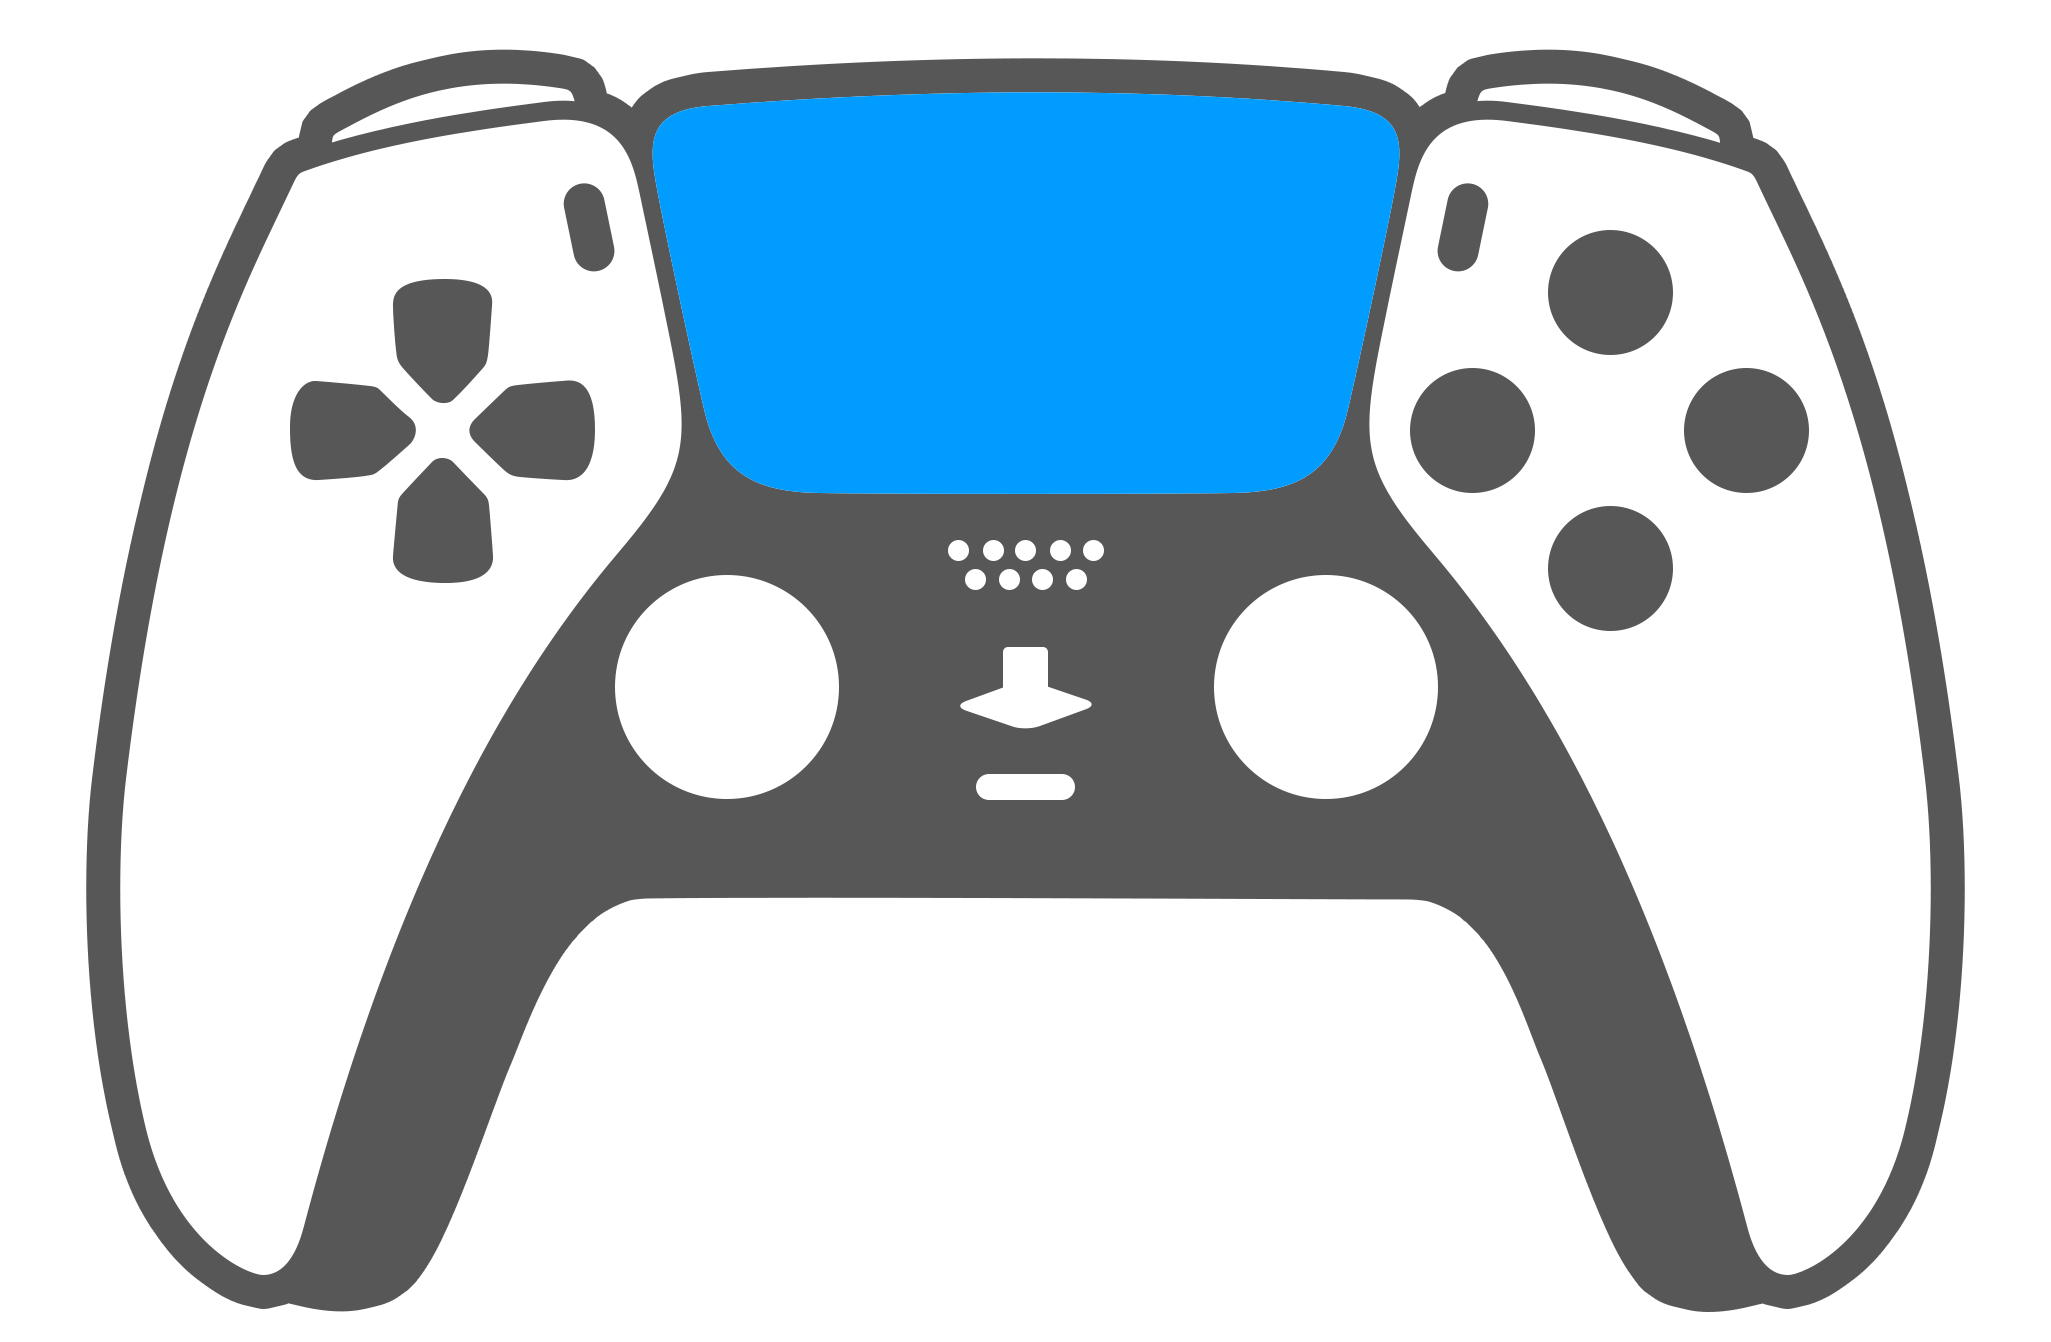
\includegraphics[width=8cm]{frontView_touch} }}
    \caption{Touch Pad}
\end{figure}

\paragraph{Accelerometer and Gyroscope}
The controller is able to measure its positional acceleration and angular velocity. Measurements are done with 16-Bit precision in all three XYZ-Axis. Make sure to implement hysteresis, dead zones and tolerances. It may also helpful to accumulate the values over multiple frame to get a more stable result but this will also increase latency.
\begin{itemize}
	\item \textbf{Accelerometer} Measures the positional acceleration (meters/second).
	\item \textbf{Gyroscope} Measures the angular velocity (degrees/second). 
\end{itemize}
These values should be calibrated in your own code base, particularly the gyroscope which usually has per axis biases.

\paragraph{Rumble motors / Haptic feedback}
The ccontroller feature two Haptic feedback devices. Thees device work similar like normal speakers, but they are not good in producing tones, they are good in producing vibration. It is possible to send an audio signal directly to those haptic speakers (However currently not supported by this API).\\
The controller supports simulating the normal soft and hard rumble motors using the haptic speakers. When using this mode both motors can be controlled with the usual 8-Bit values. The left rumble feels hard, the right one soft.

\paragraph{Integrated speaker and microphone}
Featuring two microphones and one mono speaker, the DualSense is able to produce and pickup audio. These features are not currently supported by this API, however it is possible to address these devices through Windows independently. 

\paragraph{Stereo audio jack}
Directly under the microphone is a stereo, 3.5mm audio jack. It is possible to retrieve the connection status of this jack. However, like the speaker it is currently not supported by the API.

\paragraph{Internal timer}
The DualSense controller has an inbuilt timer which can be used to more accurately integrate the data from the accelerometer and gyroscope. The timer starts when the device is connected and is measured in units of 0.33 microseconds. The value is stored as a 32-Bit unsigned integer which will overflow after roughly 72 minutes and restart from 0. This API accounts for the overflow and calculates the correct delta time when reading the input state.

\newpage